\chapter{Environment}
\label{chapter:environment}

\section{Multi-access Edge Computing}

\subsection{Far Edge Cloud}

Benefits of far edge
    - Latency
    - Allowing thin clients / offloading task to edge
    - Price and effect to environment
    - Security
    - Centralized repairment / upgrading
    - Less power consumption

\subsection{Applications}

Requirements
- SR-IOV
- NICS

- Environment in MEC application
    - How migrated?
    - Elevated privileges and other requirements compared
    - Something else?
Nokia's environment \\
Usage of KC in Nokia's environment \\






%\begin{figure}[ht]
%  \begin{center}
%    % here the width of the figure is set to 9 cm
%    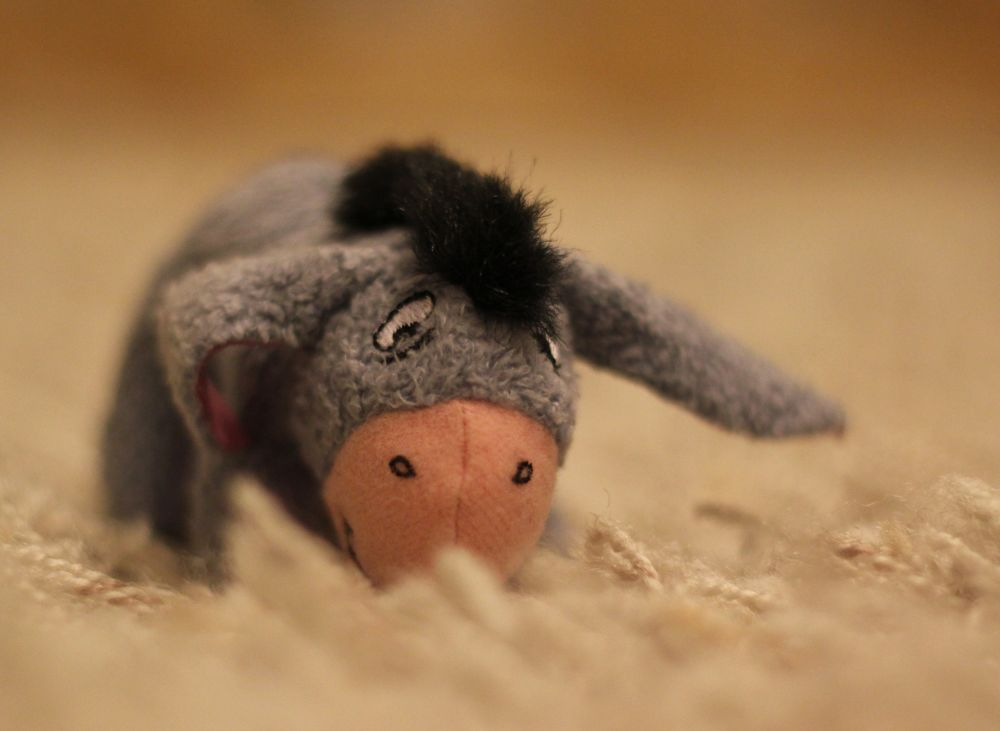
\includegraphics[width=9cm]{images/ihaa.jpg}
%    \caption{Eeyore, or Ihaa, a very sad donkey.}
%    \label{fig:eeyore}
%  \end{center}
%\end{figure}

% Comment: If your sentence ends in a capital letter write \@ before the period

% If you do need a normal space after a period (instead of
% the longer sentence separator), use \  (backslash and space) after the
% period. Like so: a.\ first item, b.\ second item.